\chapter{Sound Fields Generated by a PAL} % Main chapter title
\label{chap:sound_field} % Change X to a consecutive number; for referencing this chapter elsewhere, use \ref{ChapterX}
\blfootnote{The work presented in this chapter have been published in \cite{Zhong2020NonparaxialModelAudio, Zhong2021FieldWesterveltFar}.}

\noindent Section \ref{sec:sound_field_governing_equations} introduces the governing equations for describing the propagation of sound waves generated by a PAL.
Section \ref{sec:sound_field_quasi} proposes both the three-dimensional (3D) and two-dimensional (2D) PAL radiation models, and reviews the corresponding quasilinear solutions.
The audio sound field on front side of a baffled PAL is proposed to be divided into three regions in Sec.~\ref{sec:sound_field_front}: the near field, the Westervelt far field, and the inverse-law far field.
The reason and advantage for this division are presented.
The widely used GBE model and the convolution model are concluded in Secs.~\ref{sec:predict_gbe} and \ref{sec:predict_conv}, respectively. 
They are used to predict the audio sound in the Westervelt far field and the inverse-law far field, respectively.
Section \ref{eq:sound_field_back} investigates the audio sound field on both front and back side of a non-baffled PAL.
A non-paraxial prediction model utilizing the disk scattering theory is proposed.
Experimental results are presented to validate the proposed model.

\section{Governing equations}
\label{sec:sound_field_governing_equations}
In Westervelt's seminal work, the sound field generated by a PAL is derived from the Lighthill equation, which is expressed as \cite{Lighthill1952SoundGeneratedAerodynamically, Westervelt1963ParametricAcousticArray}
\begin{equation}
    \qty(\grad^2 - \frac{1}{c_0^2}\pdv[2]{}{t}) \tilde{\rho}
    = - \frac{1}{c_0^2}
    \pdv{}{x_i}{x_j}
    \qty[\tilde{\rho} v_i v_j - \sigma_{ij} + \qty(P-\tilde{\rho} c_0^2) \delta_{ij}]
    \label{eq:chap3:1289dfew}
\end{equation}
where $\grad^2$ is the Laplace operator, $c_0$ is the linear sound speed in air, $t$ is the time, $P$ is the ambient pressure, \revA{$\tilde{\rho}$ is the fluid density}, \revA{$\tilde{\rho} v_i v_j$} describes unsteady convection of flow (also known as Reynolds' stress), $\sigma_{ij}$ describes sound generated due to viscosity, and \revA{$(P-\tilde{\rho} c_0^2)\delta_{ij}$} represents the nonlinear acoustic generation process. 

Lighthill's equation (\ref{eq:chap3:1289dfew}) is derived from the conservation of mass and the conservation of momentum {equations} without approximations.
Combining with the equation of state and ignoring cubic and higher terms,
the second-order nonlinear wave equation is obtained as \cite{Aanonsen1984DistortionHarmonicGeneration}
\begin{equation}
    \grad^2 p - \frac{1}{c_0^2} \pdv[2]{p}{t}
    + 
    \frac{\delta}{c_0^2}\grad^2 \pdv{p}{t}
    =
    - \frac{\beta}{\rho_0c_0^4}
    \pdv[2]{ p}{t}
    - \qty(\grad^2+\frac{1}{c_0^2}\pdv[2]{}{t})\scrL
    \label{eq:chap3:1289djas12}
\end{equation}
where $p$ is the sound pressure.
The third term on the left-hand side of Eq.~(\ref{eq:chap3:1289djas12}) accounts for the fluid thermo-viscosity, where $\delta$ is the sound diffusivity parameter and this is related to the sound attenuation coefficient $\alpha$.
The first term on the right-hand side of Eq.~(\ref{eq:chap3:1289djas12}) accounts for the nonlinearity, where $\rho_0$ is the static fluid density and $\beta$ is the nonlinear coefficient; 
the second term characterizes the local non-cumulative effects, where $\scrL$ stands for the Lagrangian density and is given by 
\begin{equation}
    \scrL = \frac{\rho_0 \vb{v}\vdot \vb{v} }{2} - \frac{p^2}{2\rho_0c_0^2}
    \label{eq:lagrangian_density}
\end{equation}
where $\vb{v}$ is the acoustic particle velocity vector.

Equation (\ref{eq:chap3:1289djas12}) is time-consuming to obtain numerical results due to the evaluation of the second derivatives of the square of sound pressure $p$ and velocity $\vb{v}$ \cite{Kagawa1992FiniteElementSimulation, Cervenka2019VersatileComputationalApproach}.
The Kuznetsov equation is more often convenient to use which is equivalent to the second-order nonlinear wave equation (\ref{eq:chap3:1289djas12}) but is expressed in terms of the velocity potential, $\Phi$, \cite{Aanonsen1984DistortionHarmonicGeneration, Cervenka2019VersatileComputationalApproach}
\begin{equation}
    \grad^2 \Phi - \frac{1}{c_0^2} \pdv[2]{\Phi}{t}
     +\frac{\delta}{c_0^2} \grad^2 \pdv{\Phi}{t}
     =
    -\frac{1}{c_0^2} \pdv{}{t}\qty[(\grad\Phi)^2 + \frac{\beta-1}{c_0^2} \qty(\pdv{\Phi}{t})^2]
    \label{eq:kuznetsov_eq}
\end{equation}

The $\scrL$ term in Eq.~(\ref{eq:chap3:1289djas12}) can only produce local effects in the wave solution.
They cannot lead to cumulative effects for progressive waves which are occurred in most PAL applications.
By neglecting the Lagrangian density $\scrL$, a simpler equation (called \quotes{Westervelt equation}) is obtained as \cite{Aanonsen1984DistortionHarmonicGeneration}
\begin{equation}
    \grad^2 p - \frac{1}{c_0^2} \pdv[2]{p}{t}
    +\frac{\delta}{c_0^2}\grad^2 \pdv{p}{t}
    =
    - \frac{\beta}{\rho_0c_0^4}
    \pdv[2]{ p^2}{t}
    \label{eq:westervelt_eq}
\end{equation}

The Westervelt equation given by Eq.~(\ref{eq:westervelt_eq}) can be further simplified in the case of narrow collimated beams by utilizing the parabolic approximation for the Laplace operator $\grad^2$.
In this approximation, the second derivative along of propagation direction, i.e., the positive $z$ axis, is approximated by a first derivative. 
The KZK equation is written as \cite{Aanonsen1984DistortionHarmonicGeneration}
\begin{equation}
    \grad^2_\bot p
    - \frac{2}{c_0}\pdv{p}{z}{\tau}
      + \frac{\delta}{c_0^4}\pdv[3]{p}{\tau}
    = 
    -\frac{\beta}{\rho_0c_0^4}\pdv[2]{p^2}{\tau}
\end{equation}
where $\tau = t-z/c_0$ is the retarded time, $\grad^2_\bot = \pdv*[2]{}{x} + \pdv*[2]{}{y}$ is the transverse Laplace operator. 

\section{Quasilinear solution}
\label{sec:sound_field_quasi}
Starting from this equation, it is assumed that the ultrasound of frequencies $f_1$ and $f_2$ with condition $f_1>f_2$ is radiated by the PAL, and the average of them, i.e., $f\subt{u} = (f_1+f_2)/2$, is denoted as the carrier ultrasonic frequency.
The audio frequency is then denoted by $f\subt{a}$, which is $f_1-f_2$.
In the application of PALs, the nonlinearity is weak due to safety concerns \cite{Gan2012ReviewParametricAcoustic, Lawton2001DamageHumanHearing, Pompei2002SoundUltrasoundParametric}, so the quasilinear approximation can be safely assumed in the mathematical modelling.
By expanding the acoustic quantity up to second-order in governing equations \cite{Silva2013DifferencefrequencyGenerationNonlinear}, 
we have a set of hierarchical linear wave equations taking the form of \cite{Zhong2021FieldWesterveltFar}
\begin{equation}
    \begin{dcases}
        (\grad^2 + k_i^2) \Phi(\vb{r},k_i) = 0, i = 1,2\\
        (\grad^2+k\subt{a}^2) \Phi(\vb{r}, k\subt{a}) = q
    \end{dcases}
    \label{eq:quasilinear_eq}
\end{equation}
where the harmonic sound field is assumed, $k_i= \omega_i/c_0 + \rmi \alpha_i $ is the complex wavenumber of ultrasound, $\alpha_i$ is the ultrasound attenuation coefficient at frequency of $f_i$, $i=1,2$, \revA{$k\subt{a}=\omega\subt{a}/c_0$} is the wavenumber of audio sound, $\omega_i = 2\uppi f_i$ is the angular frequency of ultrasound, $\rmi$ is the imaginary unit, $\omega\subt{a}=2\uppi f\subt{a}$ is the angular frequency of audio sound, $\Phi(\vb{r},k)$ represents the velocity potential at the field point $\vb{r}$ of wavenumber $k$, and $q$ is the source density for audio sound. 
It can be found the ultrasound is governed by a homogeneous wave equation, 
while the audio sound is governed by a inhomogeneous one.
It can be seen that the original nonlinear problem is transformed into a combined linear problem.

The form of the source density, $q$, depends on the governing equation to be used. 
For Kuznetsov equation given by Eq.~(\ref{eq:kuznetsov_eq}), it takes the form of \cite{Cervenka2019VersatileComputationalApproach, Zhong2021FieldWesterveltFar}
\begin{equation}
    q (\vb{r})
    = \frac{\omega\subt{a}}{\rmi c_0^2}
    \qty[(\beta-1) \frac{\omega_1\omega_2}{c_0^2}\Phi(\vb{r},k_1) \Phi^*(\vb{r},k_2) + 
    \vb{v}(\vb{r},k_1)\vb{v}^*(\vb{r},k_2)]
    \label{eq:kuznetsov:source:density}
\end{equation}
where $\vb{v}(\vb{r},k_i)$ is the velocity vector at the field point $\vb{r}$ and of wavenumber $k_i$, $i=1,2$.
The sound pressure of audio sound is obtained using its second-order relationship with the velocity potential as \cite{Cervenka2019VersatileComputationalApproach}
\begin{equation}
    p(\vb{r}, k\subt{a})
    =
    \rmi  \rho_0\omega\subt{a} \Phi(\vb{r},k\subt{a})
    + \frac{\rho_0}{2}\qty[\frac{\omega_1\omega_2}{c_0^2}\Phi(\vb{r},k_1)\Phi^*(\vb{r},k_2) - \vb{v}(\vb{r},k_1)\vb{v}^*(\vb{r}, k_2)]
    \label{eq:kuznetsov_p_phi}
\end{equation}
where $\Phi(\vb{r},k\subt{a})$ is the velocity potential of audio sound.

For Westervelt equation given by Eq.~(\ref{eq:westervelt_eq}), the source density is reduced to \cite{Zhong2021FieldWesterveltFar}
\begin{equation}
    q(\vb{r}) = \frac{\beta \omega\subt{a} \omega_1\omega_2}{\rmi c_0^4}
    \Phi(\vb{r}, k_1)\Phi^*(\vb{r},k_2)
    \label{eq:source_density_westervelt}
\end{equation}
and the sound pressure is obtained directly from the linear version of Eq.~(\ref{eq:kuznetsov_p_phi}), which yields
\begin{equation}
    p(\vb{r},k\subt{a}) = \rmi \rho_0\omega\subt{a}\Phi(\vb{r},k\subt{a})
    \label{eq:pressure_potential_linear}
\end{equation}

\subsection{Three-dimensional model}
The 3D model is shown in Fig.~\ref{fig:pal3d:model}.
A circular PAL with a radius of $a$ generates two harmonic ultrasound of frequencies $f_1$ and $f_2$ ($f_1>f_2$) and the boundary condition on the transducer surface is written as
\begin{equation}
    u(\bm{\uprho}, t)
    =
    u(\bm{\uprho}, k_1) \rme^{-\rmi \omega_1 t}
    +
    u(\bm{\uprho},k_2) \rme^{-\rmi \omega_2 t}
    \label{eq:velocity_condition_3d}
\end{equation}
where $\bm{\uprho}= (x,y)$ are 2D transverse coordinates.
A rectangular coordinate system $Oxyz$ is established with its origin at the center of the PAL, and the positive $z$ axis is in the direction of the radiation axis.

\begin{figure}[h]
    \centering
    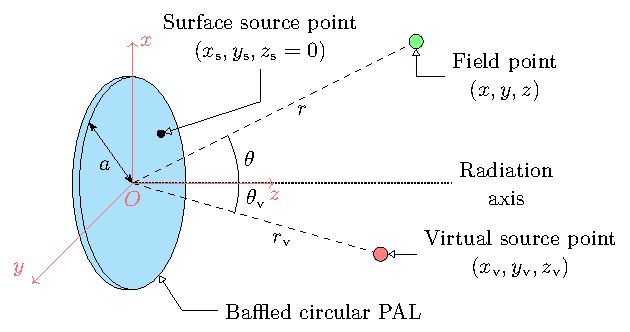
\includegraphics[width = 0.7\textwidth]{Figures/Sketch_200426.pdf}
    \caption{Sketch of a PAL and the geometric description of rectangular and spherical coordinate systems.}
    \label{fig:pal3d:model}
\end{figure}

The ultrasound field of frequency $f_i,i=1,2$, can be calculated using the Rayleigh integral \cite{Pierce2019AcousticsIntroductionIts} 
\begin{equation}
    \Phi(\vb{r}, k_i) = - 2 \iint_S 
    u(\bm{\uprho}\subt{s},k_i) 
    g(\vb{r},\vb{r}\subt{s},k_i)
    \dd^2 \bm{\uprho}\subt{s}
    \label{eq:rayleigh}
\end{equation}
where $S$ is the radiation surface area, $\bm{\uprho}\subt{s} = (x\subt{s},y\subt{s})$, $\vb{r}\subt{s} = (x\subt{s},y\subt{s},z\subt{s} = 0)$, $\dd^2\bm{\uprho}\subt{s} = \dd x\subt{s}\dd y\subt{s}$, and $g$ is the Green's function in a free field from a point $\vb{r}_1$ to a point $\vb{r}_2$ of a wavenumber of $k$, which is expressed as \cite{Pierce2019AcousticsIntroductionIts}
\begin{equation}
    g(\vb{r}_1,\vb{r}_2,k)
    =
    \frac{\rme^{\rmi k \abs{\vb{r}_1-\vb{r}_2}} }{4\uppi \abs{\vb{r}_1-\vb{r}_2}}
    \label{eq:green_function_free_field}
\end{equation}
where the Euclidean distance between the points $\vb{r}_i = (x_i,y_i,z_i), i=1,2$ is 
\begin{equation}
\abs{\vb{r}_1-\vb{r}_2}
=
\sqrt{(x_1-x_2)^2 + (y_1-y_2)^2 + (z_1-z_2)^2}
\end{equation}

It is noted Eq.~(\ref{eq:rayleigh}) is validated only when the source is baffled. 
This is usually satisfied in real applications even the PAL is non-baffled, because the ultrasonic wavelength (e.g., 8.6 mm at 40 kHz) is much smaller than the aperture size of the PAL.

The orthogonal components under the rectangular coordinate system $Oxyz$ of the velocity field $\vb{v}(\vb{r},k_i)$ for ultrasound can be obtained by using the relation $\vb{v} = \grad \Phi$ as \cite{Cervenka2019VersatileComputationalApproach}
\begin{equation}
    \begin{dcases}
        v_{x}(\vb{r}, k_i) = 
        \pdv{\Phi(\vb{r},k_i)}{x}
        = 
        \frac{1}{2\uppi}
        \iint_S 
        u (\bm{\uprho}\subt{s}, k_i)
        \frac{(x-x\subt{s})(1-\rmi k _i \abs{\vb{r}-\vb{r}\subt{s}})}{\abs{\vb{r}-\vb{r}\subt{s}}^3}\rme^{\rmi k_i\abs{\vb{r}-\vb{r}\subt{s}} }  \dd^2 \bm{\uprho}\subt{s}\\
        v_{y}(\vb{r}, k_i) = 
        \pdv{\Phi(\vb{r},k_i)}{y}
        = 
        \frac{1}{2\uppi}
        \iint_S 
        u (\bm{\uprho}\subt{s}, k_i)
        \frac{(y-y\subt{s})(1-\rmi k _i \abs{\vb{r}-\vb{r}\subt{s}})}{\abs{\vb{r}-\vb{r}\subt{s}}^3}\rme^{\rmi k_i \abs{\vb{r}-\vb{r}\subt{s}} } 
        \dd^2 \bm{\uprho}\subt{s}\\
        v_{z}(\vb{r}, k_i) = 
        \pdv{\Phi(\vb{r},k_i)}{z}
        = 
        \frac{1}{2\uppi}
        \iint_S 
        u (\bm{\uprho}\subt{s}, k_i)
        \frac{z(1-\rmi k _i \abs{\vb{r}-\vb{r}\subt{s}})}{\abs{\vb{r}-\vb{r}\subt{s}}^3}\rme^{\rmi k_i \abs{\vb{r}-\vb{r}\subt{s}} }   \dd^2\bm{\uprho} \subt{s}
    \end{dcases}
\end{equation}

The velocity potential for audio sound is then obtained according to Eq.~(\ref{eq:quasilinear_eq}) as 
\begin{equation}
    \Phi(\vb{r},k\subt{a})
    =
    -
    \iiint_V
    q(\vb{r}\subt{v})
    g(\vb{r},\vb{r}\subt{v}, k\subt{a})
    \dd^3\vb{r}\subt{v}
    \label{eq:potential_integral_volume}
\end{equation}
where $V$ represents the full space to be integrated.

The integral in Eq.~(\ref{eq:potential_integral_volume}) is singular when $\vb{r}=\vb{r}\subt{v}$. 
The following substitution can be used to eliminate the singularity
\begin{equation}
    \begin{dcases}
        x\subt{v} = r\subt{v}'\cos\varphi\subt{v}' \sin \theta\subt{v}'+x\\
        y\subt{v}  = r\subt{v}'\sin\varphi\subt{v}' \sin \theta\subt{v}'+y\\
        z\subt{v} = r\subt{v} '\cos\theta\subt{v}'+z
    \end{dcases}
\end{equation}
and Eq.~(\ref{eq:potential_integral_volume}) becomes 
\begin{equation}
    \Phi(\vb{r},k\subt{a})
    = 
    -\frac{1}{4\uppi}
    \int_{0}^{2\uppi}
    \int_0^\uppi
    \int_0^\infty
    q(\vb{r}\subt{v})
    \rme^{\rmi k \subt{a} r\subt{v}'}
    r\subt{v}' \sin\theta\subt{v}' 
    \dd r\subt{v}'
    \dd \theta\subt{v}'
    \dd\varphi\subt{v}'
    \label{eq:sdpfj}
\end{equation}
The substitution of the source density given by Eqs.~(\ref{eq:kuznetsov:source:density}) or (\ref{eq:source_density_westervelt}) into Eqs.~(\ref{eq:potential_integral_volume}) or (\ref{eq:sdpfj}), and the utilization of Eqs.~(\ref{eq:kuznetsov_p_phi}) or (\ref{eq:pressure_potential_linear}) yields the audio sound pressure. 

\subsection{Two-dimensional model}
The rectangular phased array PAL is the most common one in industrial applications. 
Due to the poor convergence of the Rayleigh integral, it is hard to directly calculate the radiation from a rectangular source. 
When one dimension of the radiation surface of a piston source is much larger than the wavelength, the radiated sound field can be approximately modelled as the radiation from infinitely long strips \cite{Mellow2011SoundFieldsInfinitely, Poletti2019CylindricalExpansionsSound}. 
After using the integral expression of the Hankel function (also known as the 2D Green's function), the two-fold Rayleigh integral can be simplified into a onefold one. 
Based on such a model, the sound field radiated by a traditional loudspeaker has been extensively studied.
In this thesis, a similar model for the PAL radiation is proposed as shown in Fig.~\ref{fig:pal2d:model}, which is denoted as 2D model.

The rectangular $(x, y, z)$ and the cylindrical $(\rho, \varphi, z)$ coordinate systems are established with their origin, $O$, at the center of the PAL and the positive $y$ axis pointing to the radiation direction, where $\rho$ and $\varphi$ are the radial and polar angle coordinates, respectively. 
It is assumed that the dimension of the PAL along the $z$ axis is infinitely long, so that only the sound field on the plane $xOy$ needs to be considered. 
The length of the phased array PAL along the $x$ axis is $2a$.

\begin{figure}[h]
    \centering
    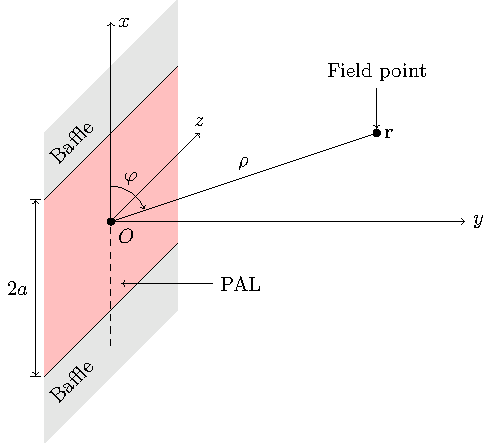
\includegraphics[width = 0.6\textwidth]{Figures/pal2d_model_210817.pdf}
    \caption{Sketch of a phased array PAL and the geometrical description of rectangular and cylindrical coordinate systems.}
    \label{fig:pal2d:model}
\end{figure}

In this model, the velocity boundary on the radiation surface is a simplification of Eq.~(\ref{eq:velocity_condition_3d}) a 
\begin{equation}
    u(x, t)
    =
    u(x, k_1) \rme^{-\rmi \omega_1 t}
    +
    u(x,k_2) \rme^{-\rmi \omega_2 t}
    \label{eq:velocity_condition_2d}
\end{equation}
The ultrasound potential can be obtained as, see \cite{Poletti2019CylindricalExpansionsSound} and Eq.~(2.46) in \cite{SchmerrJr2014FundamentalsUltrasonicPhased}
\begin{equation}
    \Phi(\bm{\uprho}, k_i) = 
    - 2 \int_{-a}^a 
    u(x\subt{s},k_i)
    g\subt{2D}(\bm{\uprho},\bm{\uprho}\subt{s},k_i)
    \dd x\subt{s}
    \label{eq:potential_2d}
\end{equation}
where $\bm{\uprho} = (x,y)$ and $\bm{\uprho}\subt{s} =(x\subt{s},y\subt{s}=0)$, and $g\subt{2D}$ is a 2D Green's function in free field
\begin{equation}
    g\subt{2D}(\bm{\uprho}_1,\bm{\uprho}_2, k) 
    =
    \frac{\rmi }{4}H_0(k\abs{\bm{\uprho}_1-\bm{\uprho}_2})
    \label{eq:green_2d_328}
\end{equation}
where $H_0(\cdot)$ is the Hankel function of first kind of order 0, and the Euclidean distance between points $\bm{\uprho}_i=(x_i,y_i), i=1,2$ is 
\begin{equation}
    \abs{\bm{\uprho}_1-\bm{\uprho}_2} = 
    \sqrt{(x_1-x_2)^2 + (y_1-y_2)^2}
\end{equation}

The components of velocity field for ultrasound $\vb{v}(\bm{\uprho}, k_i)$ are
\begin{equation}
\begin{dcases}
    v_x(\bm{\uprho},k_i)  = 
    \frac{1}{2\rmi} \int_{-a}^a 
    u(x\subt{s}, k_i) 
    \frac{k_i(x-x\subt{s})}{|\bm{\uprho}-\bm{\uprho}\subt{s}|} 
    H'_0(k_i|\bm{\uprho}-\bm{\uprho}\subt{s}|) 
    \dd x\subt{s}\\
    v_y(\bm{\uprho},k_i)  = 
    \frac{1}{2\rmi} 
    \int_{-a}^a 
    u(x\subt{s}, k_i) 
    \frac{k_iy}{|\bm{\uprho}-\bm{\uprho}\subt{s}|} 
    H'_0(k_i|\bm{\uprho}-\bm{\uprho}\subt{s}|) 
    \dd x\subt{s}\\
    v_z(\bm{\uprho},k_i) = 0
\end{dcases}
\end{equation}

The velocity potential for the audio sound is then
\begin{equation}
    \Phi(\bm{\uprho}, k\subt{a}) =
    -
    \iint_{-\infty}^\infty 
    q(\bm{\uprho}\subt{v}) 
    g\subt{2D}(\bm\rho, \bm\rho\subt{v}, k\subt{a})
    \dd^2 \bm{\uprho}\subt{v}
    \label{eq:chap3:902jfd}
\end{equation}

The Hankel function in Eq.~(\ref{eq:chap3:902jfd}) is singular when $\vb{r} = \vb{r}\subt{v}$, resulting a singular integral. 
To eliminate the singularity, the following substitutions can be used
\begin{equation}
    \begin{dcases}
        x\subt{v} = \rho\subt{v}' \cos\varphi\subt{v}' + x\\
        y\subt{v} = \rho\subt{v}'\sin\varphi\subt{v}' + y
    \end{dcases}
\end{equation}
The integral given by (\ref{eq:chap3:902jfd}) becomes
\begin{equation}
    \Phi(\bm{\uprho},k_i) 
    =
    \frac{1}{4\rmi }
    \int_0^{2\uppi} \int_0^\infty
    q(\bm{\uprho}\subt{v})
    H_0(k\subt{a}\rho'\subt{v})
    \rho'\subt{v} 
    \dd\rho'\subt{v}
    \dd \varphi'\subt{v}
\end{equation}

%% todo: sinh transformation

\section{The sound field on front side of a baffled PAL}
\label{sec:sound_field_front}
\subsection{The near field, Westervelt far field, and inverse-law far field}
The near and far fields of traditional loudspeakers are differentiated by whether the sound pressure amplitude is inversely proportional to the propagating distance in the region \cite{Foote2014DiscriminatingNearfieldFarfield}, 
but the audio sound fields generated by a PAL are more complicated due to its nonlinear nature \cite{Cervenka2019VersatileComputationalApproach}.
In this thesis, it is proposed to divide the audio sound field on front of a baffled PAL into three regions: the inverse-law far field, the Westervelt far field, and the near field. 
With this proposed classification, appropriate models can be chosen for different regions to enable faster and more accurate sound field calculation.

In the inverse-law far field, the inverse-law holds, and the solutions are the simplest. 
Starting from the Lighthill equation,
Westervelt obtained a closed-form formula for the audio sound in the inverse-law far field by assuming the ultrasound is collimated and nonlinear interactions of ultrasound take place only over a limited distance \cite{Westervelt1963ParametricAcousticArray}.
Berktay \cite{Berktay1965PossibleExploitationNonlinear} and Berktay and Leahy \cite{Berktay1974FarfieldPerformanceParametric} modified Westervelt's formula by taking into account effects arising from the cylindrical and/or spherical spreading of ultrasonic waves, 
and they improved prediction accuracy by introducing an aperture factor for the transducer and the product directivity of ultrasonic waves.
The Berktay solution is given as a simple expression in the time domain, which provides the basis for the signal modulation techniques in the realization of PALs.
Several modifications to the Berktay model were later proposed to improve the prediction accuracy for the sidelobes of PALs \cite{Shi2012ProductDirectivityModels}. 
A more accurate model has been proposed which employs the convolution of the Westervelt directivity and the ultrasonic wave directivities \cite{Shi2015ConvolutionModelComputing, Guasch2018FarfieldDirectivityParametric, Mellen1978NumericalMethodCalculating, Moffett1981NearfieldCharacteristicsParametric}.
Although the ultrasonic waves are not assumed as collimated in the convolution model, they are assumed to be exponentially attenuated along each direction, 
which is not true in practice because of the complexity in the near field of ultrasonic transducers. The boundary of the inverse-law field is often far away from the transducer \cite{Moffett1981NearfieldCharacteristicsParametric}.

The Westervelt far field is defined as the region where Westervelt equation given by Eq.~(\ref{eq:westervelt_eq}) is accurate enough, and the local effects characterized by the ultrasonic Lagrangian density given by Eq.~(\ref{eq:lagrangian_density}) are negligible. 
When the quasilinear approximation is assumed, the audio sound can be considered as the radiation from an infinitely large virtual volume source, with the source density proportional to the product of the ultrasonic pressure. 
In earlier studies, the ultrasonic beams were simply assumed to be spherically spreading with a directivity function \cite{Mellen1978NumericalMethodCalculating, Moffett1981NearfieldCharacteristicsParametric}.
Recently, the nonlinear interactions of actual ultrasonic beams generated by a transducer were modelled to improve prediction accuracy \cite{Zhong2020NonparaxialModelAudio, Zhong2020SphericalExpansionAudio}. 
To simplify the calculation, the paraxial (Fresnel) approximation is usually assumed for ultrasonic waves and this enables a Gaussian beam expansion method to be used because the ultrasonic wavelength is usually much smaller than the PAL radius \cite{Cervenka2013NonparaxialModelParametric}. 
If the paraxial approximation is assumed for both ultrasonic and audio waves, then the Westervelt equation reduces to the well known Khokhlov-Zabolotskaya-Kuznetsov (KZK) equation after approximating a second order derivative of sound pressure with respect to the propagating direction by a first order derivative. 
The calculation is further simplified, although the result is accurate only inside the paraxial region, which is inside about $20^\circ$ from the transducer axis \cite{Hamilton2008NonlinearAcoustics}.

In the near field, the local effects characterized by the ultrasonic Lagrangian density cannot be neglected. 
The audio sound pressure distribution is more complicated and local maxima and minima occur in a similar way to that observed in the near field of traditional loudspeakers. 
The general second-order nonlinear wave equation is accurate in the modelling of the near field audio sound \cite{Aanonsen1984DistortionHarmonicGeneration}.
However, its equivalent form written in terms of the velocity potential (the Kuznetsov equation), is often used because the evaluation of the second-order spatial derivatives of the ultrasonic Lagrangian density can be avoided \cite{Cervenka2019VersatileComputationalApproach, Kagawa1992FiniteElementSimulation}.
Unfortunately, the calculation of the quasilinear solution of the Kuznetsov equation is rather time-consuming, so the audio sound in the near field of PALs is rarely calculated using this equation. 
The audio sound in the near field of the PAL can also be obtained by using the direct numerical calculation of the Navier-Stokes equations in the time domain, although this again incurs heavy computational expenditure \cite{Nomura2012NumericalSimulationParametric}. 
Thus, the near field for audio sound generated by PALs is complicated and difficult to calculate, which means that it is convenient to separate out the sound pressure field and to apply different models to different regions.

Figure~\ref{fig:soundfields:289f} shows the audio SPL generated by a PAL as a function of the propagating distance at 1 kHz. 
The parameters used in simulations are presented in Table \ref{tab:param:f98fjs}.
The curves denoted by \quotes{Kuznetsov} and \quotes{Westervelt} are obtained using the Kuznetsov and Westervelt equations given by Eqs.~(\ref{eq:kuznetsov_eq}) and (\ref{eq:westervelt_eq}), repectively.
The curve denoted by \quotes{Inverse-law} is obtained by an extrapolation of the inverse-law formula according to the method described in Sec.~\ref{sec:swe_pal_inverse_law}.
Here, the results obtained by the 3 methods are different, from which the audio sound field is proposed to be divided into 3 regions.

\begin{figure}[htb]
    \centering
    \begin{subfigure}{0.7\textwidth}
        \centering
        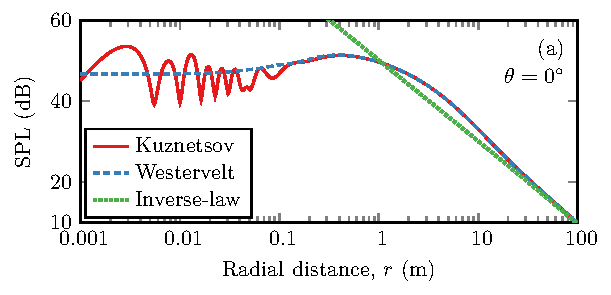
\includegraphics[width = \textwidth]{fig/fullfield_a0p05_ultra40e3_audio1000_angle0_200802H.pdf}
    \end{subfigure}
    \\
    \begin{subfigure}{0.7\textwidth}
        \centering
        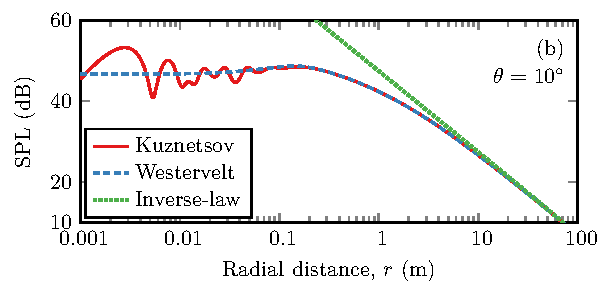
\includegraphics[width = \textwidth]{fig/fullfield_a0p05_ultra40e3_audio1000_angle10_200802J.pdf}
    \end{subfigure}
    \caption{The audio SPL \revA{(dB re 20 $\mu$Pa)} as a function of the propagating distance at 1 kHz calculated with different methods: (a) on the radiation axis ($0^\circ$), and (b) in the direction of the angle $10^\circ$. 
    The parameters in Table \ref{tab:param:f98fjs} are used.}
    \label{fig:soundfields:289f}
\end{figure}

\begin{table}
    \centering
    \begin{tabular}{ll}
        \toprule
        Item & Description \\
        \midrule
        Transducer surface radius & $a = \SI{0.05}{m}$\\
        Average ultrasonic frequency & $f\subt{u} = \SI{39.5}{kHz}$\\
        Audio frequency & $f\subt{a} = \SI{1}{kHz}$\\
        Sound attenuation coefficients & $\alpha_1=\alpha_2 = \SI{2.8e-2}{Np/m}$\\
        Helmholtz number for ultrasound & $k\subt{u} a  = 14.7$\\
        Rayleigh distance for ultrasound & $\SI{0.146}{m}$\\
        \bottomrule
    \end{tabular}
    \caption{The parameters used in the simulations.}
    \label{tab:param:f98fjs}
\end{table}

In the near field, the audio SPL is complicated and local maxima and minima take place due to strong local effects characterized by the ultrasonic Lagrangian density given by Eq.~(\ref{eq:lagrangian_density}), so the Kuznetsov equation must be used here. 
When the radial distance is larger than 0.42 m and 0.19 m in Figs.~\ref{fig:soundfields:289f}(a) and (b), respectively, 
the difference between the curves denoted by \quotes{Kuznetsov} and \quotes{Westervelt} is less than 0.1 dB, 
and so the Westervelt equation may be used to predict the audio sound in the Westervelt far field. 
The inverse-law far field is the region where the radial distance is larger than 28.7 m and 7.3 m in Figs.~\ref{fig:soundfields:289f}(a) and (b), respectively, 
and the difference between the curves denoted by \quotes{Westervelt} and \quotes{Inverse-law} is less than 1 dB
. 
The transitions from the near field to the Westervelt far field, and to the inverse-law far field will be discussed in Sec.~\ref{sec:swe_pal}.


\subsection{Gaussian beam expansion}
\label{sec:predict_gbe}
The GBE method is widely used to simplify the calculation of the radiation from a PAL.
Considering a circular radiation surface for the PAL as shown in Fig.~\ref{fig:pal3d:model}, the velocity profile is written as the superposition of $N$ Gaussian functions
\begin{equation}
    u(\rho, k_i) = 
    u_0
    \sum_{n=1}^N A_n \exp\qty(-B_n \frac{\rho^2}{a^2})
\end{equation}

If one applies the following paraxial approximation for the Green's function 
\begin{equation}
    (x_1-x\subt{2})^2 +(y_1-y\subt{2})^2  \ll (z_1-z_2)^2
\end{equation}
The one-order approximation is satisfied as \cite{Freedman1960SoundFieldRectangular, Mast2007FresnelApproximationsAcoustic}
\begin{equation}
    g(\vb{r}_1,\vb{r}_2,k ) 
    =\frac{\rme^{\rmi k \abs{\vb{r}_1-\vb{r}_2}}}{4\uppi \abs{\vb{r}_1-\vb{r}_2}}
        \approx
        \frac{1}{4\uppi \abs{z_1-z_2}}
        \exp\qty(\rmi k\qty[\abs{z_1-z_2} + \frac{(x_1-x_2)^2 +(y_1-y_2)^2 }{2\abs{z_1-z_2}}])
\end{equation}
By using the integral given by Eq.~(5) in \cite{Ding2003ExtensionsGaussianBeam},  the Rayleigh integral given by Eq.~(\ref{eq:rayleigh}) is approximated by the superposition of multiple Gaussian beams
\begin{equation}
    \Phi(\vb{r}, k_i) = 
    \frac{u_0}{\rmi k_i}
    \sum_{n=1}^N \frac{A_n}{1+\rmi B_nz/\scrR(k_i) }
    \exp\qty( \rmi k_i z - \frac{B_n}{1+\rmi B_nz/\scrR(k_i)} \frac{\rho^2}{a^2})
    \label{eq:piston:gbe}
\end{equation}
where the Rayleigh distance $\scrR(k_i) = k_ia^2/2$.
The GBE coefficients $A_n$, $B_n$, and $N$ are obtained by the heuristic method
where the transducer vibration velocity profile is approximated by the superposition of multiple ($N$) Gaussian velocity profiles. 
For a circular piston source, the expansion coefficients have been calculated for $N = 10$ \cite{Wen1988DiffractionBeamField}, $N = 15$ \cite{Huang1999GaussianFiniteelementMethod}, $N = 25$ \cite{Kim2006GenerationBasisSets}, and $N = 40$ \cite{Cervenka2015StructureMultiGaussianBeam} where larger $N$ provides more accurate results. 

Figure~\ref{fig:piston_axis_compare} compares the normalized sound pressure calculated using the GBE method and the closed-form formula, which is given by,  see Eq.~(5.7.3) in \cite{Pierce2019AcousticsIntroductionIts}
\begin{equation}
    \Phi (z,k)
    =
    -\frac{2u_0}{k}
    \exp\qty[\rmi \frac{ka}{2} \qty(\sqrt{1+\frac{z^2}{a^2}} + \frac{z}{a}) ]
    \sin\qty[\frac{ka}{2}\qty(\sqrt{1+\frac{z^2}{a^2}} -\frac{z}{a})]
    \label{eq:piston:axis:closed_form}
\end{equation}
Although the results obtained using the GBE method is inaccurate at the points near the transducer, 
the calculation error becomes negligible in the transition region and far field \cite{Wen1988DiffractionBeamField}.

\begin{figure}[htb]
    \centering
    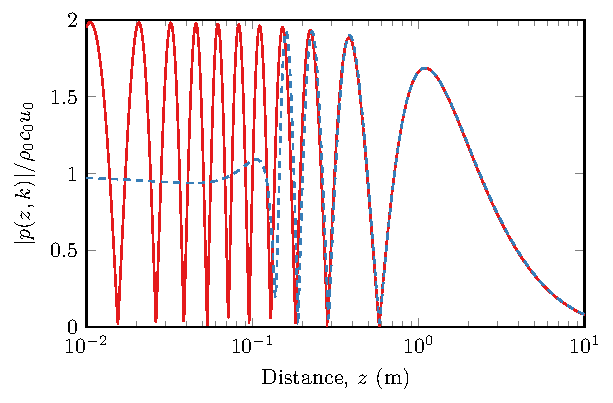
\includegraphics[width = 0.6\textwidth]{fig/CircPistonAxis_GBE_demo1_Wen1988JASA.pdf}
    \caption{Normalized sound pressure along the radiation axis. Solid line, calculated using the closed-form solution given by Eq.~(\ref{eq:piston:axis:closed_form}). Dashed line, calculated using the GBE method, where the transducer radius $a=\SI{0.1}{m}$, and the GBE coefficients are chosen from \cite{Wen1988DiffractionBeamField}.}
    \label{fig:piston_axis_compare}
\end{figure}


The substitution of Eq.~(\ref{eq:piston:gbe}) into Eq.~(\ref{eq:source_density_westervelt}) and the utilization of Eq.~(\ref{eq:pressure_potential_linear}) yields
\begin{dmath}
    q(\vb{r})
    =
    \frac{\beta\omega\subt{a} \abs{u_0}^2}{\rmi c_0^2}
    \rme^{\rmi (k_1-k_2^*) z}
    \sum_{n,m=1}^N
    \frac{A_n}{1+\rmi B_n z/\scrR(k_1)}
    \frac{A_n^*}{1-\rmi B_m^* z/\scrR^*(k_2)}
    \\ \times
    \exp\qty[-\qty(\frac{B_n}{1+\rmi B_n z/\scrR(k_1)} + 
    \frac{B_m^*}{1-\rmi B_m^* z/\scrR^*(k_2)}) \frac{\rho^2}{a^2}]
    \label{eq:f8923jfwserfsd}
\end{dmath}
By substituting Eq.~(\ref{eq:f8923jfwserfsd}) into Eq.~(\ref{eq:potential_integral_volume}), one obtains the audio sound field as 
\begin{equation}
    \Phi(\vb{r},k\subt{a})
    =
    -2\uppi
    \int_0^\uppi \int_0^\infty
    q(\vb{r}\subt{v})
    % \frac{\rme^{\rmi k\subt{a}\abs{\vb{r}-\vb{r}\subt{v}}}}{ 2\abs{\vb{r}-\vb{r}\subt{v}}}
    g(\vb{r},\vb{r}\subt{v}, k\subt{a})
    \rho\subt{v}
    \dd \rho\subt{v}\dd\theta\subt{v}
    \label{eq:sf982wf}
\end{equation}
where the symmetric property about $\varphi\subt{v}$ has been used. 

Equation (\ref{eq:sf982wf}) is referred to \quotes{non-paraxial model} in \cite{Cervenka2013NonparaxialModelParametric} because the paraxial approximation is not assumed for audio sound.
If one applies the GBE for audio sound in Eq.~(\ref{eq:sf982wf}), the so-called \quotes{paraxial solution} is obtained as 
\begin{dmath}
    \Phi(\vb{r},k\subt{a})
    =
    \frac{\beta \abs{u_0}^2 }{2c_0}
    \int_0^z
    \sum_{n,m=1}^N
    \frac{A_nA_m^*}{C_{n,1}C_{m,2}^*}
    \frac{1}{1+\rmi D_{nm} \abs{z-z\subt{v}}/\scrR(k\subt{a})}
    \\
    \times \exp\qty[\rmi (k_1-k_2^*)z\subt{v}
    + \rmi k\subt{a} \abs{z-z\subt{v}} 
    - 
\frac{D_{nm}}{1+\rmi D_{nm }\abs{z-z\subt{v}}/ \scrR(k\subt{a})} \frac{\rho^2 }{a^2}]
    \dd z\subt{v}
    \label{eq:gbe:pressure}
\end{dmath}
where
\begin{equation}
    C_{n,1} = 1+\rmi B_nz\subt{v} / \scrR(k_1)\qc
    C_{m,2} = 1+\rmi B_mz\subt{v}/\scrR(k_2)
\end{equation}
\begin{equation}
    D_{nm} 
    = \frac{B_n}{C_{n,1}} + \frac{B_m^*}{C_{n,2}^*}
\end{equation}

It is noted that Eq.~(\ref{eq:gbe:pressure}) can be used only for a circular piston source. 
The GBE model can also be used for the piston source that has other shapes, such as rectangular and elliptical \cite{Ding2003ExtensionsGaussianBeam, Ding2004NotesGaussianBeam, Ding2005SupplementaryNotesGaussian}.
The GBE model mentioned in this section is based on the assumption of paraxial approximation, some extensions on this model have been proposed which is applicable in the non-paraxial region \cite{Zhao2009NonparaxialMultiGaussianBeam, Wang2017TwodimensionalAnalyticModeling}.

\subsection{Convolution model}
\label{sec:predict_conv}
In the inverse-law far field, where the audio sound pressure is inversely proportional to the propagating distance, the expression of the audio sound can be further simplified.
The directivity for the audio sound is defined as
\begin{equation}
    \calD(\theta,k\subt{a}) 
    = 
    \abs{\frac{p(\vartheta,k\subt{a})}{p(\vartheta=0,k\subt{a})}}
\end{equation}
where $\vartheta$ is defined as the angle between the field point and the radiation axis ($\varphi = \uppi/2$ in Fig.~\ref{fig:pal2d:model}) so that $\vartheta = \abs{\varphi-\uppi/2}$. 
The convolution method assumes the field point is in the inverse-law far field, where good agreement between predictions and measurements has been shown using this method. 
This method is, therefore, used for the purpose of comparison against the proposed alternative approach and is briefly summarized here.

The directivity of the audio sound is obtained by the convolution model as
\begin{equation}
    \calD(\vartheta,k\subt{a})
    =
    \qty[\calD(\vartheta,k_1) \calD(\vartheta,k_2)]
    \ast
    \calD\subt{W} (\vartheta,k\subt{a})
    \label{eq:conv}
\end{equation}
where $\calD(\vartheta,k_1)$ and $\calD(\vartheta,k_2)$ are directivities of ultrasound, 
$\ast$ denotes the linear convolution operation,
and $\calD\subt{W}(\vartheta,k\subt{a})$ is Westervelt's directivity \cite{Westervelt1963ParametricAcousticArray}
\begin{equation}
    \calD\subt{W}(\vartheta,k\subt{a})
    =
    \frac{1}{\sqrt{1+k\subt{a}^2 \tan^4 \vartheta / (\alpha_1+\alpha_2)^2 }}
\end{equation}
The ultrasound in the convolution model is assumed to be exponentially attenuated in each direction, which is not true in reality because of the complexity of ultrasound beams in the near field of the transducers. Therefore, some discrepancies are observed between measurements and predictions in \cite{Shi2015ConvolutionModelComputing}.

\section{The sound field on back side of  a non-baffled PAL}
\label{eq:sound_field_back}
It has been reported that audible sound can be heard behind a PAL in free field \cite{Sugahara2017StudyMeasurementsAbsorption}.
However, there is no analytical model for a non-baffled PAL at present.
The finite element method (FEM) and the boundary element method (BEM) are promising techniques for solving linear acoustic problems and they are well built in much commercial simulation software. 
However, it is very difficult to compute and predict audio sound generated by non-baffled PALs directly with the existing commercial software because the model is nonlinear. 
Although the FEM model for the nonlinear sound wave propagation is available, it is time-consuming and hard to compute the sounds generated by non-baffled PALs in open space \cite{Kagawa1992FiniteElementSimulation}. 
Therefore, an analytical prediction model for non-baffled PALs is needed.

PALs are usually manufactured in circular or square shapes with small thickness, so it can be treated as a finite size disk or square plate. 
The sound scattering by a finite size disk can be solved analytically \cite{Flammer2005SpheroidalWaveFunctions, Zhong2018EffectsFiniteSize}, so the disk-shaped PAL is considered in this section. 
The solution consists of the spheroidal wave functions derived from the oblate spheroidal coordinate system. 
Although the computation of spheroidal wave functions is complicated, some software or codes are available \cite{Zhang1996ComputationSpecialFunctions, VanBuren2017AccurateCalculationOblate}. 
In this section, 
a non-paraxial model is developed for a finite size and disk-shaped PAL based on the quasilinear approximation and the disk scattering theory. 
Each virtual audio source generated by ultrasound is regarded as a point monopole so that its scattered sound by the finite size disk can be solved. 
The non-paraxial solution of total audio sounds is exact on both front and back sides of the non-baffled PAL.
The sound on both front and back sides are calculated numerically and compared with the existing non-paraxial model for the parametric source installed in an infinitely large baffle. 

\subsection{Theory}
The oblate coordinates $(\eta, \xi,\varphi)$ are related to the rectangular coordinates $(x,y,z)$ as follows \cite{Flammer2005SpheroidalWaveFunctions, Bensoam2021SelfMutualRadiation} 
\begin{equation}
    \begin{dcases}
        x = a \sqrt{(1-\eta^2)(1+\xi^2)}\cos\varphi\\
        y = a\sqrt{(1-\eta^2)(1+\xi^2)}\sin\varphi\\
        z = a\eta \xi 
    \end{dcases}
\end{equation}
where $2a$ is the focal distance.

The boundary of the disk is assumed to be rigid for audio sound, so it follows the condition
\begin{equation}
    \left. \pdv{\Phi(\vb{r},k\subt{a})}{\xi} \right|_{\xi = \xi\subt{b} = 0} = 0
\end{equation}
The total sound field for the audio sound is obtained using Eq.~(\ref{eq:potential_integral_volume}) as
\begin{equation}
    \Phi(\vb{r},k\subt{a})
    =- a^3
    \int_0^{2\uppi} \int_0^1 \int_0^\infty 
    q(\vb{r}\subt{v})
    G(\vb{r}, \vb{r}\subt{v}, k\subt{a})
    (\xi\subt{v}^2 + \eta\subt{v}^2)\dd\xi\subt{v}
    \dd \eta\subt{v}
    \dd \varphi \subt{v}
    \label{eq:disk_potential_int}
\end{equation}
where the relation $\dd x\subt{v} \dd y\subt{v}\dd z \subt{v} = a^3 (\xi\subt{v}^2+\eta\subt{v}^2)\dd \xi\subt{v}\dd\eta\subt{v} \dd \varphi\subt{v}$ is used. 
$G(\vb{r}, \vb{r}\subt{v}, k\subt{a})$ is the Green's function in the presence of a rigid disk and can be expressed as \cite{Flammer2005SpheroidalWaveFunctions}
\begin{dmath}
    G(\vb{r}_1,\vb{r}_2,k) = \frac{\rmi k }{2\uppi}
    \sum_{m=0}^\infty \sum_{n=m}^\infty
    \eps_m 
    \chi_{mn}(-\rmi k a , \rmi \xi_1, \rmi \xi\subt{2})
    S_{mn}(-\rmi k a,\eta_1) 
    S_{mn}(-\rmi k a, \eta\subt{2})
    \cos\qty[m(\varphi_1-\varphi\subt{2})]
    \label{eq:green_func_disk}
\end{dmath}
where $\eps_m$ is the Neumann factor, $\eps_m = 1$ when $m=1$, $\eps_m = 2$ when $m\neq 1$, and the radial component is 
\begin{dmath}
    \chi_{mn}(-\rmi k a,\rmi \xi_1 ,\rmi \xi_2)
    =R_{mn}^{(1)}(-\rmi ka, \rmi \xi_<)
    R_{mn}^{(3)} (-\rmi k a , \rmi \xi_>) 
    -  \frac{R_{mn}^{(1)\prime}(-\rmi k a, \rmi \xi\subt{b} )}{R_{mn}^{(3)\prime} (-\rmi k  a , \rmi \xi\subt{b} )} 
    R_{mn}^{(3)}(-\rmi k  a,\rmi \xi_1)
    R_{mn}^{(3)}(-\rmi k a ,\rmi \xi_2)
\end{dmath}
where $\vb{r}\subt{v} = (\eta\subt{v}, \xi\subt{v}, \varphi\subt{v})$ is the location of the virtual audio source in the oblate spheroidal coordinate system, $\eps_m$ is the Neumann factor i.e. $\eps_m = 1$ for $m = 0$ and $\eps_m = 2$ for $m \neq 0$, $\xi_> = \max(\xi, \xi\subt{v})$ and $\xi_< = \min(\xi, \xi\subt{v})$. 
The notations of spheroidal wave functions follow that in \cite{Zhang1996ComputationSpecialFunctions, VanBuren2017AccurateCalculationOblate}, where $S_{mn}(−\rmi k\subt{a}a, \eta)$ is the normalized angular oblate spheroidal wave function, $R_{mn}^{(i)}(-\rmi k\subt{a} a,\rmi \xi)$ and $R_{mn}^{(i)\prime}(-\rmi k\subt{a}a, \rmi \xi)$ are the $i$\mbox{-th} kind of the radial oblate spheroidal wave functions and their derivatives with respect to $\xi$, respectively, $i = 1, 3$. 
The readers may refer to \cite{Zhang1996ComputationSpecialFunctions, VanBuren2017AccurateCalculationOblate} for the computations of these special functions. 

It is hard to calculate the audio sound due to the threefold integral in Eq.~(\ref{eq:disk_potential_int}),  and the two-fold summation of Green function in Eq.~(\ref{eq:green_func_disk})
When the surface of the transducer is axisymmetric about its axis, the source density function of audio virtual sources is axisymmetric, so the total audio sound of the non-baffled model can be simplified by integrating the azimuthal angle $\varphi\subt{v}$, yielding
\begin{equation}
    \Phi(\vb{r}, k\subt{a})
    = -2\uppi a^3 
    \int_0^1 \int_0^\infty 
    q(\vb{r}\subt{v})
    G_0(\vb{r},\vb{r}\subt{v}, k\subt{a})
    (\xi\subt{v}^2 + \eta\subt{v}^2) \dd \xi\subt{v}\dd\eta\subt{v}
    \label{eq:fdai:w4efjsdofjas}
\end{equation}
where 
\begin{equation}
    G_0(\vb{r},\vb{r}\subt{v},k\subt{a})
    = \frac{\rmi k\subt{a}}{2\uppi}
    \sum_{n=0}^\infty \chi_{0n}(-\rmi k\subt{a}a, \rmi \xi, \rmi \xi\subt{v})
    S_{0n}(-\rmi k\subt{a} a ,\eta )
    S_{0n}(-\rmi k \subt{a} a,\eta\subt{v})
\end{equation}

\subsection{Results and discussions}
In this section, both simulation and experiment results are presented. 
As shown in Fig.~\ref{fig:disk_exp_setup}, the experiments were conducted in the hemi-anechoic room with dimensions of $\SI{7.20}{m} \times \SI{5.19}{m} \times \SI{6.77}{m}$ (height) and the PAL used in experiments is a Holosonics Audio Spotlight AS-24i \cite{HolosonicsAudioSpotlight24i} with a surface size of $\SI{0.6}{m} \times \SI{ 0.6}{ m}$. 
In the simulations, a circular piston was driven with a uniform surface vibration velocity amplitude and the radius was set as 0.3385 m so that its area is the same as that of the rectangular PAL used in experiments, i.e., \revA{$0.6^2$} $\approx \uppi \times 0.3385^2$.

\begin{figure}[htb]
    \centering
    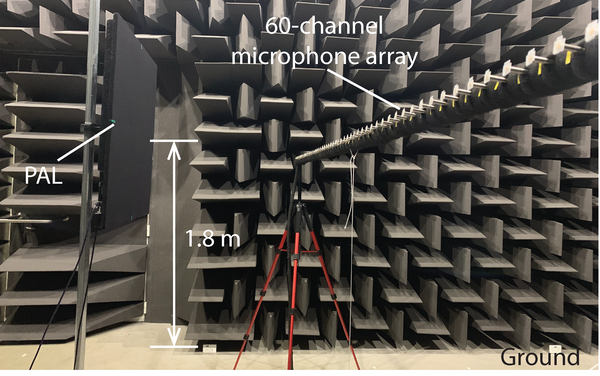
\includegraphics[width = 10cm]{fig/exp_setup_211007A_resize.png}
    \caption{The experimental setup.}
    \label{fig:disk_exp_setup}
\end{figure}

The relative humidity and the temperature in the experiments were 60\% and $25\celsius$, respectively. 
The carrier frequency of the PAL is 64 kHz measured by a Brüel \& Kjær Type 4939 microphone. 
All of the aforementioned measured data are set as known parameters in the simulations and the air absorption coefficients are calculated according to ISO 9613-1 \cite{1993ISO961311993}. 
The air absorption of audio sounds is neglected to simplify the computation of the spheroidal wave functions that are obtained by modifying the codes of \cite{VanBuren2017AccurateCalculationOblate}.

The sound field was measured at a rectangular grid with $60 \times 61 = 3661$ points in the $yOz$ plane at the height of 1.8 m. 
In all cases, 60 microphones were located in the $y$ direction from $y = \SI{-1.45}{ m}$ to $y = \SI{1.5}{m}$ with a spacing of 5 cm and they were measured simultaneously with a customary made 60-channel microphone array. 
The microphone array was located at 61 different positions in the $z$ direction from $z = \SI{-3 }{m}$ to $z = \SI{3}{m}$ with a spacing of 10 cm. 
All the measurement microphones are Brüel \& Kjær Type 4957 calibrated by Brüel \& Kjær 4231 calibrator and the sound pressure at the microphones was sampled with a Brüel \& Kjær PULSE system (the analyzer 3053-B-120 with the front panel UA-2107-120). 
The fast Fourier transform (FFT) analyzer in PULSE LabShop was used to obtain the FFT spectrum. 
To avoid the spurious sounds at microphones induced by the intensive ultrasounds radiated by the PAL, all the microphones are covered by a piece of small and thin plastic film \cite{Ji2019ExperimentalInvestigationParameters}. 
The experimental results show the insertion loss of this plastic film is more than 30 dB at 64 kHz, which is sufficient for blocking the ultrasonic sounds, and less than 0.6 dB below 1 kHz, which is negligible for the audio sound under tests.

Figure~\ref{fig:disk:we9f0sd} shows SPLs of audio sound along the $z$ axis generated by the finite size disk-shaped PAL using the baffled and non-baffled models and the experimental results. 
All SPLs in the simulations are normalized to a value so that the SPL at $z = \SI{2.0}{m}$ for the baffled PAL is the same as that measured in the experiments. 
For the audio sounds on the back side ($z < 0$), it cannot be predicted by the baffled model, so there are no data for this model. 

\begin{figure}[h]
    \centering
    % 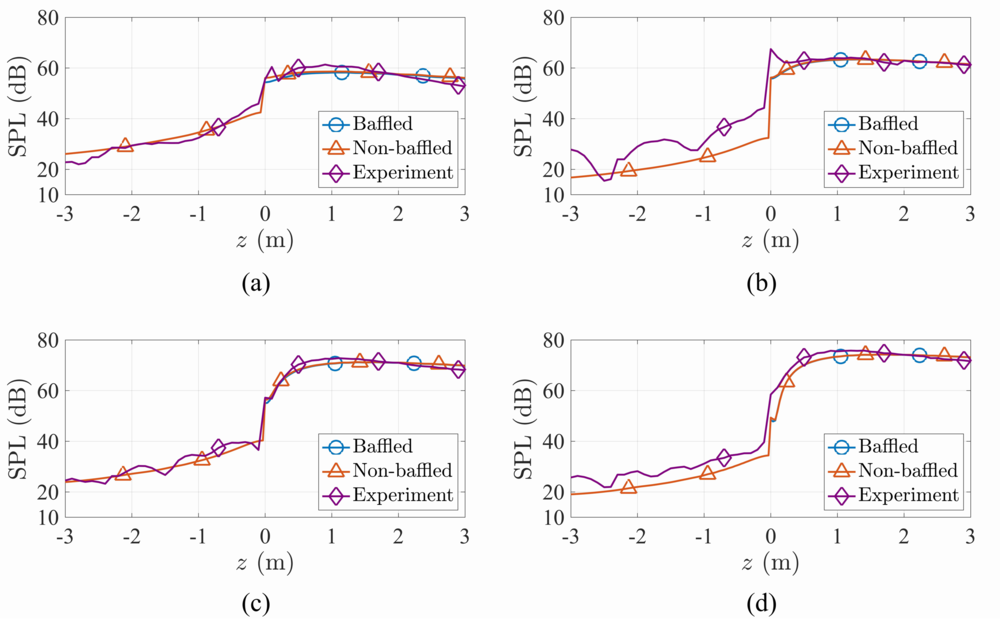
\includegraphics[width = 0.9\textwidth]{Figures/CompareAxisPrs_resize.png}
    \begin{subfigure}{0.49\textwidth}
        \centering
        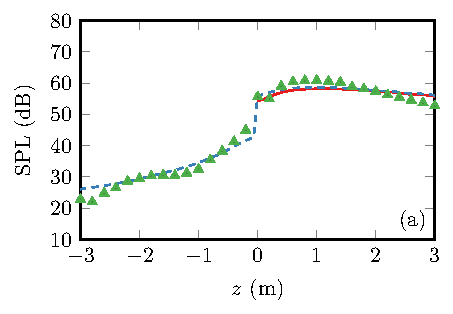
\includegraphics[width = \textwidth]{fig/CompareAxisPrs_315Hz.pdf}
    \end{subfigure}
    \begin{subfigure}{0.49\textwidth}
        \centering
        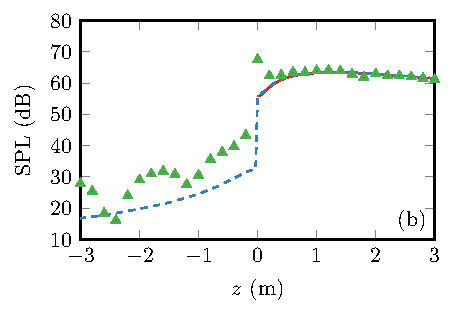
\includegraphics[width = \textwidth]{fig/CompareAxisPrs_500Hz.pdf}
    \end{subfigure}
    \\
    \begin{subfigure}{0.49\textwidth}
        \centering
        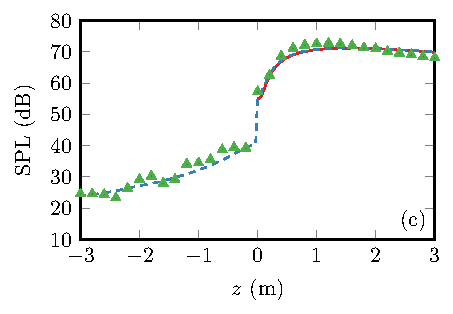
\includegraphics[width = \textwidth]{fig/CompareAxisPrs_800Hz.pdf}
    \end{subfigure}
    \begin{subfigure}{0.49\textwidth}
        \centering
        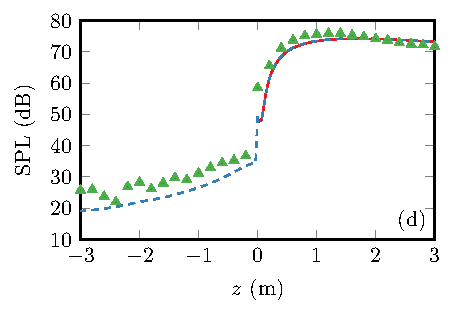
\includegraphics[width = \textwidth]{fig/CompareAxisPrs_1000Hz.pdf}
    \end{subfigure}
    \caption{Audio \revA{SPL (dB re 20 $\mu$Pa)} along the $z$ axis at different audio frequencies: (a) 315 Hz, (b) 500 Hz, (c) 800 Hz, and (d) 1 kHz. 
        \revA{Solid line, baffled model given by Eq. ({\ref{eq:potential_integral_volume}}); dashed line, non-baffled model given by Eq. ({\ref{eq:fdai:w4efjsdofjas}}); triangle, measurement.}
}
    \label{fig:disk:we9f0sd}
\end{figure}

It can be found that the values from both the models at all frequencies are almost the same at locations far away in front of the PAL, and the maximum difference is less than 0.4 dB for $z > \SI{1}{m}$. 
The experimental results on both front and back sides of the PAL are generally in accordance with those predicated by the non-baffled model. 
Large errors occur at 500 Hz when $z < \SI{0.2}{m}$ which might be caused by the measurement errors, the reflection of grounds, the shape of the PAL, and the scattering effects of the equipment.

The curves of SPL for the non-baffled PAL at $z = \SI{-0.1}{m}, \SI{0.25}{m}, \SI{-0.5}{m}, \SI{-1.0}{m}$, and $\SI{-2.0}{m}$ at different frequencies are shown in Fig.~\ref{fig:disk:123489}. 
The surface SPL of ultrasounds, i.e. the level of $\rho_0c_0\abs{v_i}$, $i = 1, 2$, is set as 125 dB at all curves for better comparison. 
Both Figs.~\ref{fig:disk:we9f0sd} and \ref{fig:disk:123489} demonstrate that there are audible audio sounds on the back side of the PAL which is caused by the diffracting of the finite size disk. 
For example, the SPL is 45 dB at $z = \SI{- 0.1 }{m}$ at 315 Hz while the audio sound at $z = \SI{1.0}{m}$ in front of the PAL is about 61.4 dB.

\begin{figure}[htb]
    \centering
    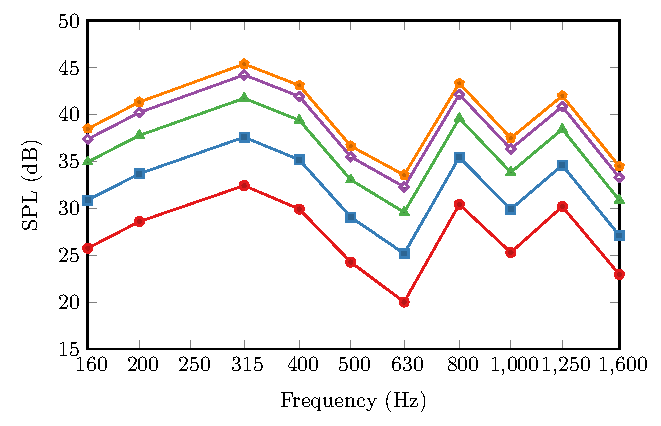
\includegraphics[width = 9cm]{fig/CompareSplOctave.pdf}
    \caption{Audio \revA{SPL (dB re 20 $\mu$Pa)} along the $z$ axis obtained using the non-baffled model at 1/3 octave center frequencies from 160 Hz to 1.6 kHz when the surface SPL of ultrasound is 125 dB. 
    Red circle, $z=\SI{-2}{m}$; Blue square, $z=\SI{-1}{m}$; green triangle, $z =\SI{-0.5}{m}$; purple diamond, $z=\SI{-0.25}{m}$; orange pentagon, $z=\SI{-0.1}{m}$.}
    \label{fig:disk:123489}
\end{figure}

\begin{figure}[H]
    \centering
    % 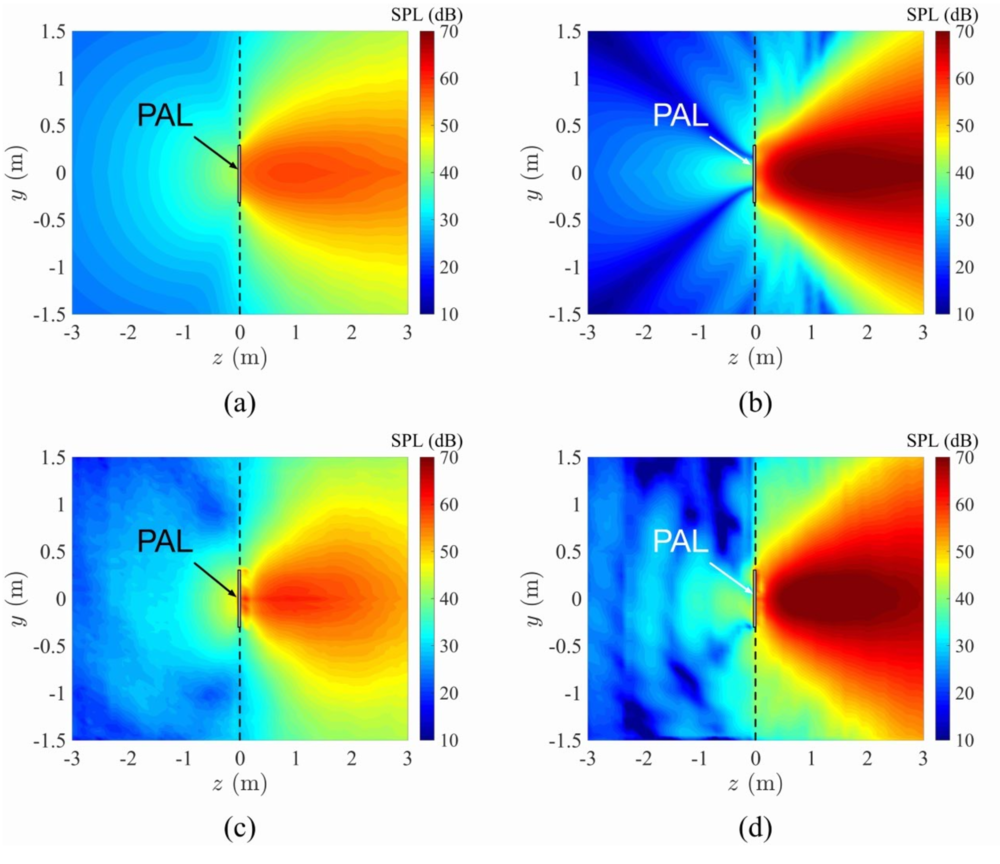
\includegraphics[width = 0.8\textwidth]{Figures/ComparePalAudio2D_resize.png}
    \begin{subfigure}{0.49\textwidth}
        \centering
        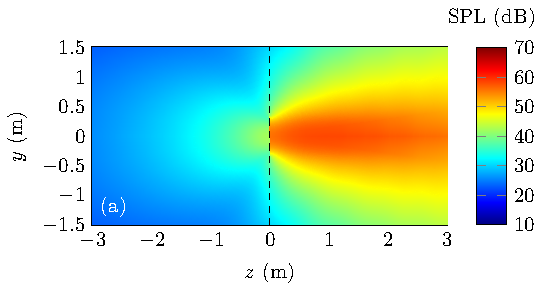
\includegraphics[width = \textwidth]{fig/ComparePalAudio2D_Simulation_315Hz.pdf}
    \end{subfigure}
    \begin{subfigure}{0.49\textwidth}
        \centering
        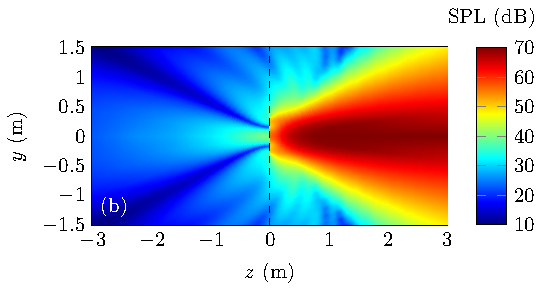
\includegraphics[width = \textwidth]{fig/ComparePalAudio2D_Simulation_800Hz.pdf}
    \end{subfigure}
    \\
    \begin{subfigure}{0.49\textwidth}
        \centering
        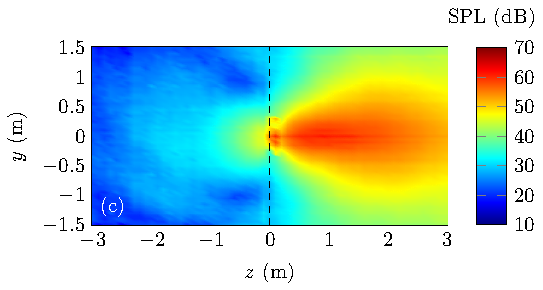
\includegraphics[width = \textwidth]{fig/ComparePalAudio2D_Experiment_315Hz.pdf}
    \end{subfigure}
    \begin{subfigure}{0.49\textwidth}
        \centering
        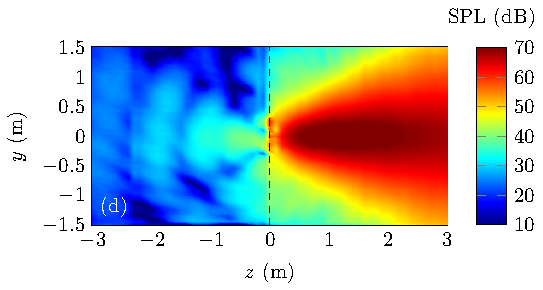
\includegraphics[width = \textwidth]{fig/ComparePalAudio2D_Experiment_800Hz.pdf}
    \end{subfigure}
    \caption{Audio \revA{SPL (dB re 20 $\mu$Pa)} predicated by the proposed non-baffled model at (a) 315 Hz and (b) 800 Hz; and the measurements at (c) 315 Hz and (d) 800 Hz. The PAL is placed at the origin and the radiation surface is on the plane $z=0$, denoted by the dashed line.}
    \label{fig:disk_2d_results}
\end{figure}

The SPL is largest at 315 Hz (the wavelength is 1.09 m) for all cases because the constructive interference of waves is largest for point monopoles when the radius of the PAL is approximately 0.35 times of the wavelength \cite{Zhong2018EffectsFiniteSize}.
As the frequency decreases from 315 Hz, the SPL on the back side decreases due to the fact that the frequency response of the PAL decreases significantly (12 dB) as the audio frequency is halved \cite{Bennett1975ParametricArrayAir}. 
As the frequency increases from 315 Hz, the SPL on the back side decreases firstly and then reaches the local maxima at 800 Hz and 1250 Hz because the diffraction effects are weakened firstly as the wavelength becomes smaller until it reaches other resonant frequencies where the constructive interference of waves is significant. 

The SPL distribution in $yOz$ plane at 315 Hz and 800 Hz are shown in Fig.~\ref{fig:disk_2d_results}, where the simulation and experiment results agree well, so the sound fields on the back side of the PAL can be well predicated by the proposed non-baffled model. 
\revA{There are some resonances in the measured sound fields which is caused by the concrete ground floor in experiments.} 
It is also found that the audio sound is audible over a large area on the back side of the PAL. 
For example, at 315 Hz, there is an approximately circular region centered at the PAL with the radius of about 1.3 m where the SPLs are more than 35 dB. 
Therefore, the effects of the finite size of the PAL should be taken into account.


\section{Summary}
The governing equations including the Lighthill equation, second-order nonlinear wave equation, Kuznetsov equation, Westervelt equation, and KZK equation, are introduced in Sec.~\ref{sec:sound_field_governing_equations}.
The quasilinear solutions for both Kuznetsov and Westervelt equations are both obtained using the successive method in Sec.~\ref{sec:sound_field_quasi}.
Both the 3D and 2D models for a PAL were proposed, and the corresponding solutions are found to be a five-fold and three-fold integrals, respectively.
The difficulty is the simplification of the numerical calculations for these integrals in the mathematical modelling.

 In Sec.~\ref{sec:sound_field_front}, the sound field is proposed to be divided into 3 regions: the near field, the Westervelt far field, and the inverse-law far field, according to the properties of audio sound on front side of a baffled PAL.
 The near field is defined as the region where the local effects cannot be neglected, so that the Kuznetsov equation given by Eq.~(\ref{eq:kuznetsov_eq}) should be used.   
The Westervelt far field is defined as the region where Westervelt equation given by Eq.~(\ref{eq:westervelt_eq}) is accurate enough, and the local effects characterized by the ultrasonic Lagrangian density given by Eq.~(\ref{eq:lagrangian_density}) are negligible. 
Many existing methods, such as the GBE method introduced in Sec.~\ref{sec:predict_gbe}, aim to obtain numerical results in the Westrevelt far field.
The inverse-law far field is the region where the audio sound pressure is inversely proportional to the propagation distance. 
The most existing accurate model in this region is the convolution model, which is introduce in Sec.~\ref{sec:predict_conv}.

A non-paraxial model for the radiation of a non-baffled PAL in free field is developed in Sec.~\ref{eq:sound_field_back} based on the quasilinear approximation and the disk scattering theory. 
In this model, each virtual audio source generated by the ultrasound in space is regarded as a point monopole and its scattered sound by a finite size disk is computed. 
Both simulation and experiment results demonstrate that audible audio sound exists on back side of the PAL, indicating that the effects of the finite size of the PAL should be taken into account when calculating the low frequency audio sound field.
